\documentclass{article}

\usepackage[final]{style}
\usepackage[utf8]{inputenc} % allow utf-8 input
\usepackage[T1]{fontenc}    % use 8-bit T1 fonts
\usepackage{hyperref}       % hyperlinks
\usepackage{url}            % simple URL typesetting
\usepackage{booktabs}       % professional-quality tables
\usepackage{amsfonts}       % blackboard math symbols
\usepackage{nicefrac}       % compact symbols for 1/2, etc.
\usepackage{microtype}      % microtypography
\usepackage{verbatim}
\usepackage{graphicx}       % for figures
\usepackage{amsmath}
\usepackage{tikz}

\makeatletter
\def\idots{\mathinner{\mkern1mu\raise\p@
\vbox{\kern7\p@\hbox{.}}\mkern2mu
\raise4\p@\hbox{.}\mkern2mu\raise7\p@\hbox{.}\mkern1mu}}
\makeatother

\title{Lecture \#4: Pixels and Filters}

\author{
  Brian Hicks, Alec Arshavsky, Sam Trautwein, Christine Phan, James Ortiz \\
  Department of Computer Science\\
  Stanford University\\
  Stanford, CA 94305 \\
  \texttt{\{bhicks2, arshava, rodion1, cxphan, jameso2\}@cs.stanford.edu} \\
}

\begin{document}

\maketitle


\emph{\textbf{Contents:}}
\begin{enumerate}
  \item Image Sampling and Quantization
  \item Image Histograms
  \item Images as Functions
  \item Linear Systems
  \item Convolution and Correlation
\end{enumerate}




\section{Image Sampling and Quantization}

\subsection{Image Types}
\paragraph{Binary Images} 
        contain pixels that are either black (0) or white (1).
			\paragraph{Grayscale Images} have a wider range of intensity than black and white. Each pixel is a shade of gray with pixel values ranging between 0 (white) and 255 (black). 
			\paragraph{Color Images} have multiple channels with colors (RGB, LAB, HSV). Each pixel in a channel are values 0-255 for intensity.  
            A 3D \emph{tensor} usually represents color images (Width x Length x 3), where the 3 channels can represent RGB, LAB, HSV, and so on.
         
		
	\subsection{Sampling and Resolution}
    Images are \textbf{samples}: they are not continuous, they are discrete pixels of a certain size and density. This can lead to errors (or graininess) because we can only measure with a certain resolution and must approximate.
			
\paragraph{Resolution} is a sampling parameter, defined in dots per inch. The standard DPI value for screens is 72 DPI.
\begin{figure}[h!]
\begin{center}
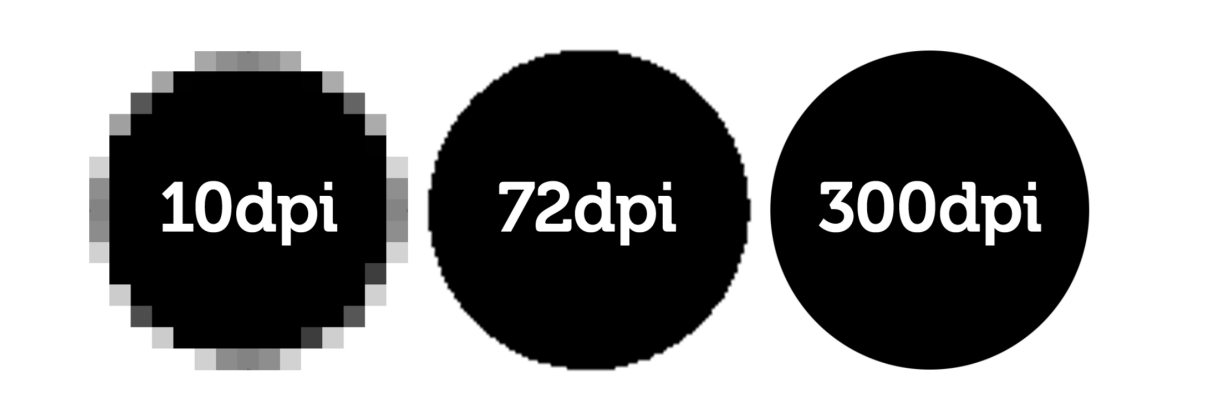
\includegraphics[scale=0.4]{res.png} \\
\caption{Illustrations of different pixel densities. Taken from the accompanying lecture slides. (Slide 14, slide credit Ulas Bagci)
            }
\end{center}
\end{figure}

				\paragraph{Pixels} are quantized (i.e, all pixels (or channels of a pixel) have one of a set numbers of values (usually [0, 255]). Quantization and sampling loses information due to a finite precision.

\section{Image Histograms}
Histograms measure the frequency of brightness within the image: how many times does a particular pixel value appear in an image. \\

\begin{figure}[h!]
\begin{center}
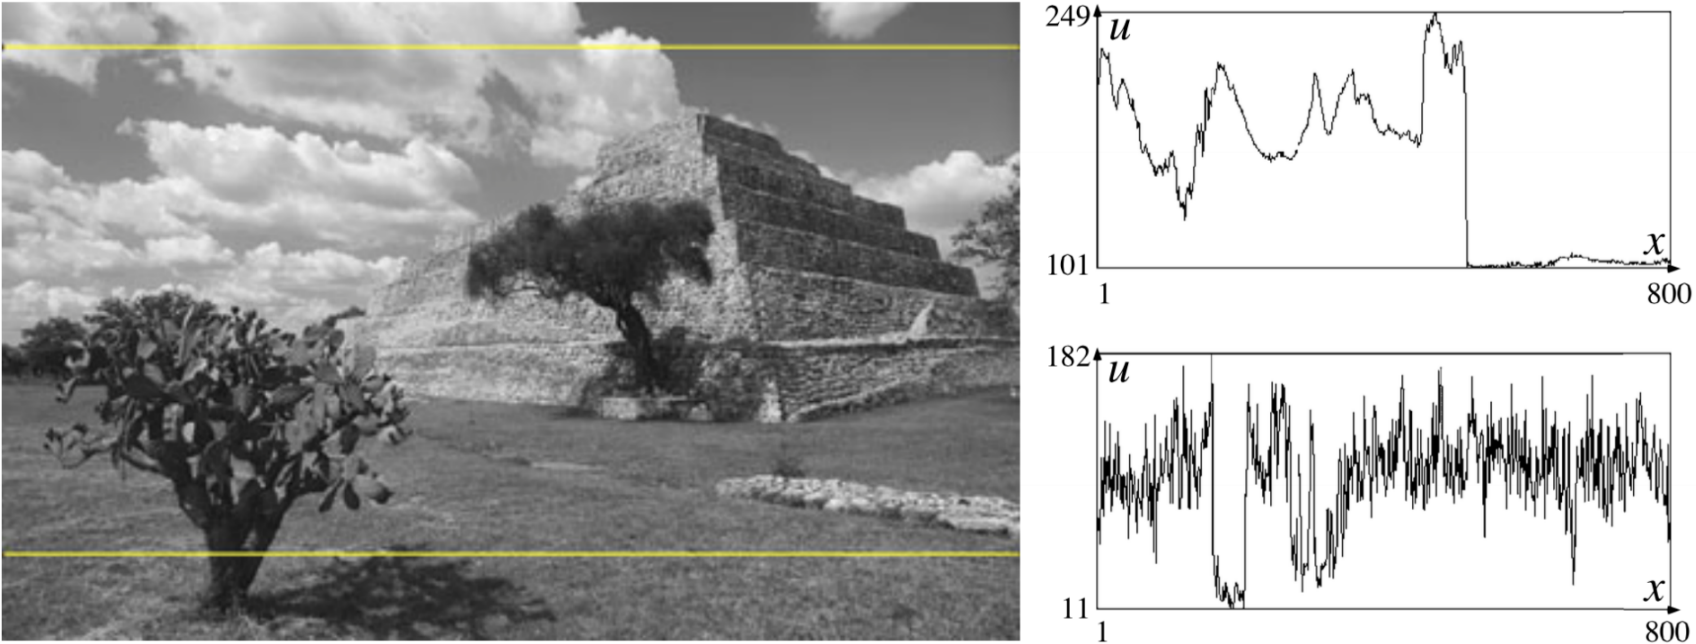
\includegraphics[scale=0.4]{histogram.png} \\
\caption{The image is sampled at two vertical positions, sampling a patch of sky and sampling a patch of grass. The corresponding histograms are shown to the right. Taken from the accompanying lecture slide (Slide 23, slide credit Dr. Mubarak Shah}
\end{center}
\end{figure}

Histograms can help us detect particular features in images, for example:
\begin{itemize}
\item Sky: Smooth coloration denotes consistency in image, consistent with the image of a sky.
\item Grass: A jagged histogram shows wide ranging variety in coloration, consistent with the shadows of a grass field. 
\item Faces: The color composition of a face will be displayed in a histogram.
\end{itemize}

An image histogram measures the frequency of certain grayscale intensities in an image. Histograms can be used to start to build up an idea of what things look like, which can be useful for classifiers.
			
            
\section{Images as Functions}

Most images that we deal with in computer vision are digital, which means that they are discrete representations of the scene shown. This discretization is achieved through the sampling of 2-dimensional space onto a regular grid, eventually producing a representation of the image as a matrix of integer values.

When dealing with images, we can imagine the image matrix as infinitely tall and wide. However, the displayed image is only a finite subset of this infinite matrix. When we deal conceive of images in this way, we can write write them as coordinates in a matrix 
\[
	\begin{bmatrix}
    	\ddots &  & \vdots & & \idots \\
        & f[-1, 1] & f[0, 1] & f[1, 1] \\
        \dots & f[-1, 0] & f[0, 0] & f[0, 1] & \dots\\
        & f[-1, -1] & f[0, -1] & f[1, -1] & \dots \\
        \idots & & \vdots & & \ddots
    \end{bmatrix}
\]
We can also treat an image as a function $f : \mathbb{R}^{2} \to \mathbb{R}^{N}$. When we do so, $f[n, m]$ where $f[n , m]$ is the intensity of a pixel at position (m, n). Note that we use square brackets, rather than the typical parentheses, to denote discrete functions.

When we treat an image as a function, it is defined over a rectangle with finite range. For example, the following function $f$ returns the (grayscale) intensity of a single pixel in an image located between $a$ and $b$ horizontally and $c$ and $d$ vertically.
\[
	f: [a, b] \times [c, d] \to [0, 255] \tag{Grayscale Pixel Intensity} 
\]
The set of values $[a, b] \times [c, d]$ is known as the \emph{domain support}, and contains all values that are valid inputs to the function $f$, while $[0, 255]$ (in this case) is the range, which defines the set of possible outputs.

We can also treat color images as a function mapping $\mathbb{R}^{2} \to \mathbb{R}^3$. For example the RGB intensities of a given pixel can be written as the function $g$ below
\[
	g[x, y] = \begin{bmatrix} r[x, y] \\ g[x, y] \\ b[x, y] \end{bmatrix} \tag{Color Pixel Intensity}
\]
where $r, g, b: [a, b] \times [c, d] \to [0, 255]$.

\section{Linear Systems (Filters)}

The term \emph{filtering} refers to a process that forms a new image whose pixel values are transformations of the original pixel values. In general, our purpose in applying filters is to extract useful information (e.g., edge detection) or else change its visual properties (e.g., de-noising).

\begin{figure}
\begin{center}
	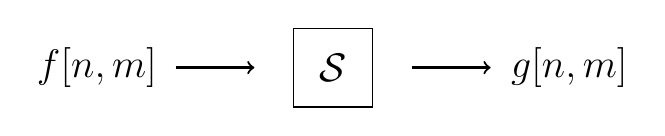
\begin{tikzpicture}
		\draw (0, 0) node {\Large $f[n, m]$};
        \draw[->, thick] (1, 0) -- (2, 0);
        \draw (2.5, 0.5) rectangle (3.5, -0.5);
        \draw (3, 0) node {\Large $\mathcal{S}$};
        \draw[->, thick] (4, 0) -- (5, 0);
        \draw (6, 0) node {\Large $g[n, m]$};
	\end{tikzpicture}
\end{center}
\caption{Graphical representation of a system's mapping of $f$ to $g$}
\end{figure}

Filters are examples of \emph{systems}, which are units that convert an input function $f[m, n]$ to an output (or response) function $g[m, n]$ where $m, n$ are the independent variables. When dealing with images, $m, n$ are the representation of a spatial position in the image.

Notationally, $\mathcal{S}$ is referred to as the \emph{system operator}, which maps a member of the set of possible outputs $g[m, n]$ to a member of the set of possible inputs $f[m, n]$. When using notation involving $\mathcal{S}$, we can write write that 
\[
\mathcal{S}[g] = f
\]
\[
	\mathcal{S}\left\{f[m, n]\right\} = g[m, n]
\]
\[
	f[m, n] \xrightarrow{\mathcal{S}} g[m, n]
\]

\subsection{Examples of Filters}

\subsubsection*{Moving Average}
One intuitive example of a filter is the \emph{moving average}. This filter sets the value of a pixel to be the average of the nine pixels in a $3 \times 3$ radius around it. Mathematically, we can represent this as
\[
	g[m, n] = \frac{1}{9} \sum\limits_{i = -1}^{1}\sum\limits_{j = -1}^{1} f[m - i, n - j] \tag{Weighted Average}
\]
This weighted average filter serves to smooth out the sharper edges of the image, creating a blurred or smoothed effect.

\subsubsection*{Image Segmentation}
We can also use filters to perform rudimentary \emph{image segmentation} based on a simple threshold system. In this case, the filter sets the value of a pixel either to an extremely high or an extremely low value, depending on whether or not it meets the threshold $t$. Mathematically, we write this as
\[
	g[m, n] = \begin{cases} 255 & f[m, n] \geq t \\ 0 & \text{otherwise}\end{cases} \tag{Threshold}
\]
Roughly speaking, this basic image segmentation filter breaks divides an image's pixels into binary classifications of bright regions and dark regions, depending on whether or not the $f[m, n] \geq t$.

\subsection{Properties of Systems}

When discussing specific systems, it is useful to be able to describe their properties. The following includes a list of properties that a system \emph{may} possess, but not all systems will have all (or any) of these properties. In other words, these are potential characteristics of individual systems, not traits of a systems in general.

\subsubsection*{Amplitude Properties}

\begin{itemize}
	\item \emph{Additivity}: A system is additive if it satisfies the equation
    \[
    	\mathcal{S}[f_i[m, n] + f_j[m, n]] = \mathcal{S}[f_i[m, n]] + \mathcal{S}[f_j[m, n]]
    \]
    
    \item  \emph{Homogeneity}: A system is homogeneous if it satisfies the equation 
    \[
		\mathcal{S}[\alpha f_i[n, m]] = \alpha\mathcal{S}[f_i[n, m]
    \]
	
    \item \emph{Superposition}: A system has the property of superposition if it satisfies the equation 
    \[
    	\mathcal{S}[\alpha f_i[n, m]] + \beta f_j[n, m]] = \alpha\mathcal{S}[f_i[n, m]] + \beta\mathcal{S}f_j[n, m]]
    \]
    
	\item \emph{Stability}: A system is stable if it satisfies the inequality 
    \[
    	\left\vert f[n, m] \right\vert \leq k \Longrightarrow \left\vert	g[n, m] \right\vert \leq ck
    \]
    for some $c$.
	
    \item \emph{Invertibility}: A system is invertible if it satisfies the equation
    \[
    	\mathcal{S}^{-1}[\mathcal{S}[f[n, m]]] = f[n, m]
    \]
\end{itemize}

\subsubsection*{Spatial Properties}

\begin{itemize}
	\item \emph{Causality}: A system is causal if for $m < m_0$ and $n < n_0$
    \[
    	f[m, n] = 0 \Longrightarrow g[m, n] = 0
    \]
    
    \item \emph{Shift Invariance}: A system is shift invariant if
    \[
    	f[m - m_0, n - n_0] \xrightarrow{\mathcal{S}} g[m - m_0, n - n_0]
    \]    
\end{itemize}

\subsection{Linear Systems}

A \emph{linear system} is a system that satisfies the property of superposition. When we employ a linear system for filtering, we create a new image whose pixels are weighted sums of the original pixel values, using the same set of weights for each pixel. A \emph{linear shift-invariant system} is a linear system that is also shift invariant. 

Linear systems also have what is known as an \emph{impulse response}. To determine the impulse response of a system $\mathcal{S}$, consider first $\delta_2[m, n]$. This is a function defined as follows
\[
	\delta_2[m, n] = \begin{cases} 1 & m = 0 \text{and} n = 0 \\
    0 & \text{otherwise} \\
    \end{cases}
\]
The impulse response $r$ is then simply
\[
	r = \mathcal{S}[\delta_2]
\]

A simple linear shift-invariant system is a system that shifts the pixels of an image, based on the shifting property of the delta function.
\[
	f[m, n] = \sum\limits_{i = -\infty}^{\infty}\sum\limits_{j = -\infty}^{\infty} f[i, j] \delta_2[m - i, n - j]
\]
We can then use the superposition property to write \emph{any} linear shift-invariant system as a weighted sum of such shifting system
\[
	\alpha_1\sum\limits_{i = -\infty}^{\infty}\sum\limits_{j = -\infty}^{\infty} f[i, j] \delta_{2,1}[m - i, n - j] + \alpha_{2,2}\sum\limits_{i = -\infty}^{\infty}\sum\limits_{j = -\infty}^{\infty} f[i, j] \delta_{2,3}[m - i, n - j] + \dots
\]
We then define the filter $h$ of a linear shift-invariant system as 
\[
	h[m, n] = \alpha_1\delta_{2,1}[m - i, n - j] + \alpha_2\delta_{2,2}[m - i, n - j] + \dots
\]


Impulse response (for all linear systems)
Delta[n,m] function: has value that is 1 specifically at one pixel, gives back a response, h[n,m]
A shifted delta function gives back a shifted response

Linear shift invariant systems (LSI)
Example: a moving average filter is a summation of impulse responses


\begin{itemize}
		\item Systems that satisfy the superposition property
		\item Have an \emph{impulse response}: $\mathcal{S}[\delta_2[n, m]] = \delta_2[{n, m}]$
		
		\item Discrete convolution: $f[n, m] * h[n, m]$ (multiplication of shifted-version of impulse response by original function)
	\end{itemize}
    
\section{Convolution and Correlation}

\subsection{Convolution}

The easiest way to think of convolution is as a system that uses information from neighboring pixels to filter the target pixel. A good example of this is a moving average, or box filter that we talked about earlier.

Convolution is represented by *, for example: \\
$f[n,m]$*$h[n,m]$
represents a function being multiplied by a shifted impulse response


Convolution allows us to compute the output of passing any input signal through a system simply by considering the impulse response of the system. To understand what this means, we must first understand how to break up a signal into a set of impulse functions.

The impulse (delta) function, $\delta [n]$, is defined to be 1 at $n = 0$ and 0 elsewhere. As seen in the image below, any signal can be decomposed as the weighted sum of impulse functions.



\begin{figure}[h!]
\begin{center}
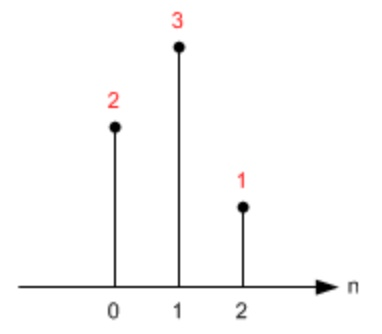
\includegraphics[scale=0.4]{input_signal_.jpeg} \\
$x[n] = x[0]\delta [n] + x[1]\delta [n-1] + x[2]\delta [n-2]$ \\
\caption{An example decomposition of a signal into an impulse function. (Adapted from http://www.songho.ca/dsp/convolution/convolution.html)}
\end{center}
\end{figure}


More generally, an arbitrary signal $x$ can be written as $x[n] = \sum_{k = -\infty}^{\infty} x[k]\delta[n-k]$.

The impulse response of a system, $h[n]$, is defined as the output resulting from passing an impulse function into a system. When a system is linear, scaling the impulse function causes the impulse response to be scaled by the same amount. Moreover, when the system is shift-invariant, shifting the impulse function causes the impulse response to be shifted by the same amount. The image below illustrates these properties for a signal consisting of 3 components. 


\begin{figure}[h!]
\begin{center}
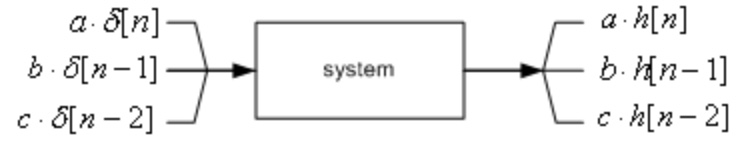
\includegraphics[scale=0.4]{impulse_response.jpeg}
\caption{An impulse function is sent through a system to create an impulse response function. Adapted from http://www.songho.ca/dsp/convolution/convolution.html}
\end{center}
\end{figure}


More generally, for an arbitrary input signal $x[n] = \sum_{k = -\infty}^{\infty} x[k]\delta[n-k]$ passed into a linear, shift-invariant system, the output is $y[n] = \sum_{k = -\infty}^{\infty} x[k]h[n-k]$, i.e. the convolution of the signal $x$ with the impulse response $h$.  

Convolution can also be done in 2 dimensions. For example, when an arbitrary, 2D signal $x[n, m] = \sum_{i = -\infty}^{\infty}\sum_{j = -\infty}^{\infty} x[i, j]\delta[n-i, m-j]$ is passed into a linear, shift-invariant system, the output is $y[n,m] = \sum_{i = -\infty}^{\infty}\sum_{j = -\infty}^{\infty} x[i, j]h[n-i, m-j]$, i.e. the convolution of the signal $x$ with the impulse response $h$ in 2 dimensions. 


\subsection{Correlation}

Cross correlation is the same as convolution, except that the filter kernel is not flipped. Two-dimensional cross correlation is represented as: \\
$r[k,l] = \sum_{m=-\infty} ^\infty \sum_{n=-\infty} ^\infty f[m+k, n+l]g[m, n]$\\
It can be used to find known features in images by using a kernel that contains target features. 



\subsubsection*{Acknowledgments}
We would like to acknowledge Professor Niebles and Krishna and the rest of the teach staff for compiling the invaluable accompanying lecture slides and delivering such an informative lecture. 


% References
\small
%\bibliographystyle{plain}

%\bibliography{bibliography}

\end{document}
